\section{Sequence Alignments}

In this section we introduce the sequence alignment problem, basic algorithms
for computing optimal alignments of two sequences.

Parts of two sequences are homologous, if they have evolved from same sequence
in their common ancestor. Aim of sequence alignment is to identify homologous
sequences. Sequences can be modified by different evolution events:
mutation of a residue into another residue, deletion of a part of the sequence,
insertion of residues into the sequence. There are also large-scale
rearrangement events like duplications (some subsequence is duplicated and
copied into other part of the sequence), inversions (some subsequence is
reversed) or translocations in which part of the sequence change position.  We will
ignore them in this thesis, as they cannot be represented by traditional
alignments. An alignment is a data structure that represents comparisons of two
or more sequences. We obtain an alignment of $k$ sequences by inserting dashes
into individual sequences so that they have the same length. We can represent an
alignment as a matrix or a table. Each row of the alignment is a sequence with
inserted dashes, and each column is a list of residues from all rows at the same
position.


An alignment has the following biological meaning: homologous residues (those that
have evolved from a common ancestor) are in same column. Dashes represents
either the parts of sequence that were deleted during evolution (deletions) or
positions where some residues were inserted into some other sequence
(insertions). In an alignment it is not possible to distinguish between insertions and
deletions -- we cannot tell if something was inserted into one sequence or if
there was deletion in the other sequences. Therefore we will refer to insertions
and deletions as to \firstUseOf{indels}.

\begin{example} 
Consider the  following evolutionary history of hypothetical DNA sequences of two
current organisms $X$ and $Y$. There was a parent sequence $P$ which evolved into
$X'$ and $Y'$ and after that $X'$ evolved into $X$ and $Y'$ evolves into $Y$.
These sequences are shown bellow: 
\begin{verbatim}
X:      C C     G C G A C C T T G C             A C C A
X':     C C     G           T T G C             A G C A
P:      A C T G G           T C G C T G A G C T A G C A
Y':     T C T G G           C C           G C T A G C A
Y:      T C T A G           C C           G A T A G C A
\end{verbatim}
%$X$ and $Y$ evolved from parent sequence $P$ through sequences $X'$ and $Y'$.
During evolution from $P$ to $X'$, four events occurred: deletion of 
sequences ``TG''  and ``TGAGCT'' and mutations of two bases. During evolution
from $X'$ to $X$, one base was changed and sequence ``CGACC'' was inserted.  
Similarly during evolution from $P$ to $Y'$, the two bases mutated and two
sequences were deleted. During evolution from $Y'$ to $Y$ one base mutated and
sequence ``CGACC'' was inserted. 

From evolutionary history described above, we can create an alignment of current
sequences $X$ and $Y$ by removing ancestral sequences $X',Y'$ and $P$, 
removing columns that contain only gaps and
replacing gaps with dashes (gap symbols). 
\begin{verbatim}
X:      C C - - G C G A C C T T G C - - - A C C A
Y:      T C T A G - - - - - C C - - G A T A G C A
\end{verbatim}
In this alignment, symbols that are in the same column are truly homologous (they
evolved from the same symbol in $P$).
As you can see, homologous symbols do not have to be equal.
\end{example}

There is only one alignment that reflects the true evolutionary history. Our goal
is to find this alignment, or at least some alignment, which is as close as
possible. The alignment shown above is a \firstUseOf{global alignment} because it
is an alignment of whole sequences $X$ and $Y$. A \firstUseOf{local alignment}
is an alignment of parts of sequences: a local alignment of sequences $X$ and
$Y$ is a global alignment of strings $\bar{X}$ and $\bar{Y}$ where $\bar{X}$ is
a substring of $X$ and $\bar{Y}$ is a substring of $Y$.  Since global
alignments do not consider rearrangement events\footnote{Duplication, reversal
or translocation.}, local alignments are useful to align sequence parts that
did not underwent such events. We will mostly consider global alignments, but
most of the methods can be extended also to local alignments.

In this section we will review basic methods for constructing alignments. We
will discuss basic scoring schemes and algorithms that find optimal alignment
under these schemes. In this thesis we cover mostly probabilistic methods.

\subsection{Scoring Schemes}

Since we want to construct alignments that have biological meaning, we have to
develop a method for assessing the quality of an alignment. One way of doing so
is to define a scoring scheme, which assigns to every alignment a real number
(called score). The alignments similar to the true alignment should have higher
score than the alignments that differ from the true alignment. Once we have a
scoring scheme, we will search for the alignment of the input sequences with
the highest score.

Typical scoring schemes used in practice score each column of
an alignment without gaps independently. Gaps are scored by a penalty
that depends on the length of the gap (the number of consecutive dashes). Score
of an entire alignment is the sum of the scores of all ungapped columns plus the
sum of the scores of all gaps.

In particular
we will assume that all sequences are from a finite alphabet $\Sigma$. For DNA,
$\Sigma=\{A,C,G,T\}$, for proteins $\Sigma$ contains $20$ codes of amino acids.
We will score a column containing residues $a$ and $b$ by $S[a,b]$ where $S$ is
a matrix of size $|\Sigma|\times|\Sigma|$ called \firstUseOf{substitution
matrix}.  A gap of length $x$ has a score $g+dx$, where $g$ is the gap opening
penalty and $d$ is the gap extension penalty. Both are usually negative, since we
want alignments that contains many columns with same or similar symbols. With
positive gap penalty there will be tendency towards alignments with many gaps
which reduce the number of aligned residues.  We call this gap scoring scheme an
affine gap model \cite{Durbin1998}. 

Matrices and gap penalties used as scoring schemes are usually derived from
frequencies of the substitutions and indels of real alignments. Example of such
matrices are PAM or BLOSUM matrices\cite{Durbin1998}. Additionally, scoring
matrices can be also derived from theoretical models of evolution, one such
example is Jukes-Cantor model\cite{Durbin1998}.

\subsection{Needleman-Wunsch algorithm}
\label{SECTION:NEEDLE}


The
alignment with the highest score can be found by the Needleman-Wunsch algorithm \cite{Durbin1998}.
This algorithm uses an arbitrary score table $S$, affine gap model with gap penalty
$d$ and gap opening penalty $g=0$ (if $g=0$ then this model is also called
linear gap model). To align sequences $X$ and $Y$ of length $n$ and $m$
respectively, we define matrix $M$ of size $n\times m$. Element $M[i,j]$ will be the
score of the best alignment of sequences $X[:i]$ and $Y[:j]$. We can compute
$M[i,j]$ by the following equations:

\begin{align} 
M[-1,-1] &= 0\\
M[-1,i] &= i\cdot d, 0< i < m\\\
M[i,-1] &= i\cdot d, 0< i < n\\
M[i,j] &= \max
\begin{cases}
 M[i-1,j-1]+S(X_i,X_j)\\M[i,j-1]+d\\
 M[i-1,j]+d
\end{cases}, 0\leq i<n,0\leq j<m \label{ALIGN:ALGO:AFFINE}
\end{align}

By computing $M[n-1,m-1]$, we have the score of the optimal (highest-scoring) alignment of $X$ and $Y$ \cite{Durbin1998}. 

To cope with gap opening penalty, we have to slightly change the algorithm.
We define two other matrices $M_X$ and $M_Y$ of same size as $M$. $M_X[i,j]$
will contain the highest score of an alignment of sequences $X[:i]$ and $Y[:j]$
that ends
with a gap in sequence $X$. $M_Y$ is analogous. Values of these matrices can be computed by the following recurrences.

\begin{align}
M[-1,-1] &= 0\\
M[-1,i] &= M_X[-1,i] = i\cdot d+g, 0 < i < m\\
M[i,-1] &= M_Y[i,-1] = i\cdot d+g, 0 < i < n\\
M_X[i,-1] &= -\infty, 0\leq i< n\\
M_Y[-1,i] &= -\infty, 0 \leq i< m\\
M[i,j] &= \max
\begin{cases}\label{ALIGN:ALGO:REALAFFINESTART}
 M[i-1,j-1]+S(X_i,X_j)\\
 M_X[i,j]\\
 M_Y[i,j]
\end{cases}, 0\leq i<n,0\leq j<m\\
M_X[i,j] &= \max
\begin{cases}
M[i-1,j]+g+d\\
M_X[i-1,j]+d
\end{cases}, 0\leq i<n,0\leq j<m\\
M_Y[i,j] &= \max
\begin{cases}
M[i,j-1]+g+d\\
M_Y[i,j-1]+d
\end{cases}, 0\leq i<n,0\leq j<m\label{ALIGN:ALGO:REALAFFINEEND}
\end{align}

To compute the
value of $M[i,j]$ (and optionally $M_X$ and $M_Y$), these equations use only values
from neighbouring cells which have at least one coordinate smaller. 
Therefore we can order computation so that when we compute value $M[i,j]$ the
necessary values are already computed.
Let $F$ be
the function, that takes as input matrix $M$  and coordinates $(i,j)$ and computes $M[i,j]$ according equation
\ref{ALIGN:ALGO:AFFINE}.  Let $F'$ be the
same function as $F$, but with $\max$ replaced with $\arg\max$.  Function
$F'(M,(i,j))$ will thus return which cell was used in computation of $F(M,(i,j))$.
Note that if $g$ is not zero, then $F$ would take as input the matrices $M,M_X,$
and $M_Y$ and compute $M[i,j],M_X[i,j],$ and $M_Y[i,j]$ according 
 equations
\ref{ALIGN:ALGO:REALAFFINESTART}-\ref{ALIGN:ALGO:REALAFFINEEND}

The Needleman-Wunsch algorithm can be implemented by the following code. For simplicity 
we show only computation of matrix $M$.

\lstset{showstringspaces=false}
%\vbox{
\begin{lstlisting}
Initialize M[i,-1] and M[-1,i]
for i in 0...n-1
  for j in 0...m-1
    M[i,j] = F(M,(i,j))
(i,j) = (n-1,m-1)
while i > 0 or j > 0
  (i',j') = F'(M,(i,j))
  (a,b) = (X[i],Y[j])
  if i' = i then a = '-'
  if j' = j then b = '-'
  print column of alignment (a,b)
  (i,j) = (i',j')
\end{lstlisting}
%}

Lines 2-5 fills matrix $M$ and lines 6-12 implement the back-tracing procedure.
Time complexity of this algorithm is $O(mn)$ and memory requirements are $O(mn)$
since we keep matrix $M$ in memory. The algorithm for
affine gap model with $g\not=0$ has the same complexity.


Note that for computing  $i$-th row of matrix $M$ we need only values from row
$i$ and $i-1$. Therefore if we want to know just the score of the optimal
alignment,
we can compute it in $O(m+n)$ memory: after computing of row $i$, we can discard
row $i-1$. However if we want find the optimal alignment, we have to keep matrix
$M$ in the memory or use one of the techniques that are described in Section 
\ref{SECTION:ALGORITHMICIMPROVEMENTS}.

\section{Sequence Alignments with Pair HMM}\label{SECTION:ALIGNWITHPHMM}

In this section we describe \abbreviation{pair hidden Markov models}{pHMM},
which are commonly used for studying relationships between different sequences,
relation between Needleman-Wunsch and pHMM, three standard decoding methods for
decoding pHMMs, and survey of literature for examples of using pHMM for
sequence alignments. 

\subsection{Pair Hidden Markov Models}\label{SECTION:PAIRHMM}

Pair hidden Markov models are HMMs that generate output on two tapes, resulting
in two emitted sequences.  Every state can in one step generate one symbol in
each sequence, or one symbol in one of the sequences or no symbols at all.
Formally, every state generates a pair of strings $(a,b)$, where $a$ and $b$
are of length at most one.  Moreover, all pairs with generated with nonzero
probability by one state have the same length.  Formal definition of pair HMMs
is given below. We can use pHMM to define probabilistic scoring schemes for
alignments.

In particular, symbols generated by the same state are considered homologous
(are in same column of an alignment). Symbols that are generated by a state
that generates only in one sequence are aligned to a gap. 

\begin{definition}
A \abbreviation{pair hidden Markov model}{pHMM} is a tuple $H=(\Sigma,V,I,d,e,a)$, where $\Sigma$ is a finite
alphabet, $V$ is a finite set of states, $I$ is an initial distribution and $a$ is
a transition matrix, all defined as
in definition \ref{DEF:HMM}. $d^x_v$ and $d^y_v$ are state durations of state $v$
in sequence $x$ and $y$ respectively. For all $v\in V$,
$d^x_v\in \{0,1\}$ and $d^y_v\in \{0,1\}$.
Emission probability matrix $e$ is
a $|V|\times\left(|\Sigma\cup\{\varepsilon\}|\right)^2$ matrix with the following
properties:
\def\lala#1{\{#1\}}
\begin{enumerate}[itemsep=-1mm]
\item
$\forall v\in V\forall \sigma_1,\sigma_2\in\Sigma\cup\{\varepsilon\}:
0\leq e_{v,(\sigma_1,\sigma_2)}\leq 1$

\item 
$\forall v\in V:
\sum_{\sigma_1,\sigma_2\in\Sigma\cup \lala{\varepsilon }}e_{v,(\sigma_1,\sigma_2)} = 1$

\item For all states $v$ if $e_{(v,\sigma_1,\sigma_2)}>0$ then
$d^x_v=|\sigma_1|$ and $d^y_v=|\sigma_2|$
\end{enumerate}

\end{definition}

A state path is defined the same as for HMMs with silent states. Restriction on
the state durations (condition $3$ in the definition) ensures that given a
state path $\pi$ and emitted sequence $X$ and $Y$, for every symbol from $X$
and $Y$ we can assign a state from $\pi$ that generated that symbol.  However,
given only two sequences $X$ and $Y$ and no state path, it is not possible to
determine which symbols of the two sequences were generated together.


\begin{definition}
Let $\pi=\pi_0\dots\pi_l$ be a state path. Then the \firstUseOf{cumulative duration
times} are
$D^x_i(\pi)=\sum_{j=0}^{i}d^x_{\pi_j}$ and $D^y_i(\pi)=\sum_{j=0}^{i}=d^y_{\pi_j}$.
Additionally, $D^x_{-1}(\pi)=D^y_{-1}(\pi)=0$. If it will be clear from the context
which state path we are using, we will write $D^x_i$ and $D^y_i$ instead of
$D^x_i(\pi)$ and $D^y_i(\pi)$.
\end{definition}

Given sequences $X,Y$ and state path $\pi$ that generated them, we 
can tell which symbols were generated by which states. Since every state $v$
generates exactly $d^x_v$ and $d^y_v$ symbols in $X$ and $Y$ respectively,
state $\pi_i$ generated pair $(X[D^x_{i-1}:D^x_{i}],Y[D^y_{i-1}:D^y_{i}])$
States $\pi_0,\pi_1,\dots\pi_{i-1}$ generated first $D^x_{i-1}$ symbols in $X$
and first $D^y_{i-1}$ symbols in $Y$. 


\begin{example}
In the figure \ref{FIGURE:SIMPLEPHMM} is pair hidden Markov model modeling
sequence alignment with affine gap model. State $M$ is called match state and
generates pair of aligned residues and corresponds to matrix $M$ from the sequence
alignment algorithm. Insert states $I_X$ and $I_Y$ represents gaps,
generates residues in only one sequence and corresponds to matrices $M_X$ and
$M_Y$ from the sequence alignment algorithm from section \ref{SECTION:NEEDLE}.

Note that a state path uniquely define an annotation (match state corresponds to
match columns, insert states represent gap).  Finding the most probable state
path for this HMM is equivalent to the Needleman-Wunsch algorithm with affine gap
model \cite{Durbin1998}.

\begin{figure}
\begin{center}
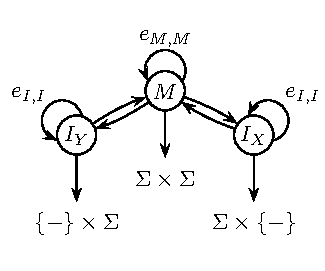
\includegraphics{../figures/pairHMM.pdf}
\end{center}
\caption[Simple pair HMM model for alignment]{Pair hidden Markov model for
pairwise alignment. It has two transitions
parameters $e_{M,M}$ and $e_{I,I}$, since we set $e_{I,M} = 1 - e_{I,I}$ and
$e_{M,I}=\frac12-\frac12e_{M,M}$. Match state $M$ generates aligned pair of symbols
and states $I_X$ and $I_Y$ generates symbols only in $X$ or $Y$ respectively.
Initial distribution is uniform.
}\label{FIGURE:SIMPLEPHMM}
\end{figure}

\end{example}

\begin{definition}
Let $H=(\Sigma,V,I,d,e,a)$ be  a pHMM, $X$ and $Y$ be arbitrary sequences over
$\Sigma$ and $\pi$ be a state path. The probability that sequences $X$ and $Y$
were generated by a model $H$  with state path $\pi$ is
\begin{equation}
\Pr\left(X,Y,\pi\mid H\right)=
I_{\pi_0}
\left(
	\prod_{i=1}^{|\pi|}a_{\pi_{i-1},\pi_i}
\right)
\left(
	\prod_{i=0}^{|\pi|}e_{\pi_i,(X[D^x_{i-1}:D^x_{i}],Y[D^y_{i-1}:D^y_{i}])}
\right)
\end{equation}
If $D^x_{|\pi|-1}\not=|X|$ or $D^y_{|\pi|-1}\not=|Y|$ then
$\Pr\left(X,Y,\pi\mid H\right)=0$. 
\end{definition}

Similarly as for HMMs, we can define the probability that sequences $X$ and $Y$ were
generated by the model $H$.

\begin{definition}
Let $H=(\Sigma,V,I,e,a)$ be a pHMM and  $X$ and $Y$ be arbitrary sequences over
$\Sigma$. Then probability that sequences $X$ and $Y$ were generated together by
model $H$ is 
\begin{equation}
\Pr\left(X,Y\mid H\right)=\sum_{\pi}\Pr\left(X,Y,\pi\mid H\right)
\end{equation}
\end{definition}


\subsection{Viterbi algorithm for pair HMM}
\label{SECTION:PAIRHMMVITERBI}
Algorithms operating over pHMMs are similar to those for the regular HMMs, but
in general they have higher computational complexity because they combine
computation  over model states with sequence alignment.  In this section, we
describe two-dimensional version of the Viterbi algorithm, other algorithms are
analogous.

The Viterbi algorithm for HMMs computes variables $V[i,v]$ and $B[i,v]$. Every
variable is parametrized by a position in the sequence and a state. For
two-dimensional version, we will add position in the second sequence.

Let $V[i,j,v]$ be the probability of the most probable state path that generated
$X[:i+1]$ and $Y[:j+1]$ and ended in state $v$. Clearly, $\max_{v\in
V}V[|X|-1,|Y|-1,v]$ is the probability of the most probable state path that
generated $X$ and $Y$. Let $B[i,j,v]$ be the last but one state of the most
probable state path that generated $X[:i+1]$ and $Y[:j+1]$ and ended in state
$v$. To make it easier, we expect that all states but one are not silent -- they emit
symbol in at least one sequence. The one silent state $s$ (start state) will have $I_s=1$.
 Let $n=|X|$ and $m=|Y|$.


\begin{align}
V[-1,-1,s] &= 1\\
V[-2,i,v] &= V[j,-2,v] = 0, \forall v\in V,-1 \leq i < n, -1\leq j < m\\
V[i,j,v] &= \max_{u\in
V}V[i-d^x_{v},j-d^y_v,u]a_{u,v}e_{v,(X[i-d^x_v:i],Y[j-d^y_v:j])}\label{EQUATION:2DVITERBIF}\\
%V[-1,j,v] &= V[i,0,v] = 0 \\
%V[0,0,v] &= I_{v}e_{v,(?,?)} \\
B[i,j,v] &= \arg\max_{u\in
V}V[i-d^x_{v},j-d^y_v,u]a_{u,v}e_{v,(X[i-d^x_v:i],Y[j-d^y_v:j])}\label{EQUATION:2DVITERBIB}
\end{align}

In equations \ref{EQUATION:2DVITERBIF} and \ref{EQUATION:2DVITERBIB} boundaries for $i$ and $j$ are $
-1\leq i< n,-1\leq j< m$ and $i>-1$ or $j>-1$.


By finding the last state $v$ of the most probable state path and back-tracing
from $B[n-1,m-1,v]$ we can reconstruct the most probable state path. Time
complexity of this algorithm is $O(nm|V|^2)$ (or $O(nm(|V|+t)$ where $t$ is the
number of transitions of $H$) and memory requirements are $O(nm|V|)$. However,
we can use various tricks to decrease memory requirements of such algorithms, as
shown in the section \ref{SECTION:ALGORITHMICIMPROVEMENTS}.

The Forward algorithm for GpHMM can be obtained by replacing maximum with
addition for computation of $V[i,j,v]$ term. The table $B$ is irrelevant for
the Forward algorithm. The Backward algorithm and Forward-Backward algorithm
are analogous to the Forward algorithm and their versions for HMM.

\subsection{Generalized Pair HMMs}\label{SECTION:GPHMM}


A \abbreviation{generalized pair HMM}{GpHMM} (or pair hidden semi-Markov
process) are combination of HMM and GHMM. Every state generates two
duration lengths $d^x$ and $d^y$ from some joint distribution associated with
the current state $d_v(d^x,d^y)$ and after that it generates two strings $x'$
and $y'$ with lengths $d^x$ and $d^y$ according to the joint distribution
$e_{v,(x',y')}$. This probability distribution can by defined for example by
pair hidden Markov model.  As with GHMMs and unlike pHMMs, the state path is not
sufficient to determine which parts of the sequences were generated by which
state, we also need two sequences of durations.
The Viterbi equations for the GpHMM are following:
\begin{align}
V[-1,-1,s] &= 1\\
V[-2,i,v] &= V[j,-2,v] = 0, \forall v\in V,-1 \leq i < n, -1\leq j < m\\
V[i,j,v] &= \max_{u\in
V,d^x\leq i, d^y\leq j}V[i-d^x,j-d^y,u]a_{u,v}e_{v,(X[i-d^x:i],Y[j-d^y:j])}d_v(d^x,d^y)\label{EQUATION:2DVITERBIFGP}\\
B[i,j,v] &= \arg\max_{u\in
V,d^x\leq i, d^y\leq j}V[i-d^x,j-d^y,u]a_{u,v}e_{v,(X[i-d^x:i],Y[j-d^y:j])}d_v(d^x,d^y)\label{EQUATION:2DVITERBIBGP}
\end{align}

In equations \ref{EQUATION:2DVITERBIFGP} and \ref{EQUATION:2DVITERBIBGP}
boundaries for $i$ and $j$ are $ -1\leq i< n,-1\leq j< m$ and $i>-1$ or $j>-1$.
Additionally, in all equations $d_x$ and $d_y$ can be also bounded by $D$, the
maximum duration length.

Drawback of GpHMM is increased computational complexity. Assume that the
emission probability can be computed in $f(n',m')$ time, where $n'$ and $m'$
are the lengths of the emitted sequences. Then the time complexity of the
Viterbi algorithm is $O(nm|E|D^2f(D,D))$ where $E$ is the set of all
transitions in a pHMM and $D$ is the maximum duration length \cite{Meyer2002}.
In the case there is not maximum duration length, the time complexity of the
Viterbi algorithm is $O(n^2m^2|E|f(n,m))$. For example, if the emission
probability is computed by another pHMM with $t$ transitions, then
$f(n',m')=O(n'm't)$ and the time complexity of the Viterbi algorithm is
$O(n^3m^3|E|t)$ or $O(nm|E|D^4t)$.  GpHMMs were successfully used for
gene-finding \cite{SLAM2003,Alexanderson2004,Majoros2005,Meyer2002}. 

The Forward algorithm, and the Forward-Backward algorithm are very similar to
their versions for pHMM. We will discuss some implementation details for these
algorithms in Sections \ref{SECTION:REPDECODING} and
\ref{SECTION:REPOPT}.

\subsection{Decoding Methods}\label{SECTION:ALNDECODING}

In this section we review three decoding methods that were used in literature to
reconstruct pairwise alignments: the Viterbi algorithm, the Posterior
decoding and the Marginalized posterior decoding.

Let $H$ be an pHMM (or GpHMM) and $X$ and $Y$ be the sequences that we want to
align. The probability $\prob{X,Y\mid H}$ is the probability that $X$ and $Y$
were generated in model $H$.  From state path $\pi$ in a pHMM  we can
reconstruct a unique alignment $A_{\pi}$. The model defines the probability 
that
$A_{\pi}$ is the true alignment of $X$ and $Y$ under the assumption, that $X$ and $Y$ were
generated by model $H$:
  \[\prob{\pi\mid
X,Y,H}=\frac{\prob{\pi,X,Y\mid H}}{\prob{X,Y\mid H}}\]
  We can use $\prob{\pi\mid X,Y,H}$ as a score of 
alignment $A_{\pi}$. Path $\pi$ with the highest score can be found by a
two-dimensional version of the Viterbi
algorithm (section \ref{SECTION:PAIRHMMVITERBI}). Alignment $A_{\pi}$ can be
constructed from $X,Y$ and $\pi$ in a straightforward
way: for every match state from $\pi$ that generated $X[i]$ and $Y[j]$ we add
column $(X[i],Y[j])$. For every indel state in $\pi$ that generates $X[i]$ we
add to alignment column $(X[i],'-')$. An indel states for the second sequences are
analogous.  The two-dimensional Viterbi algorithm is used in  most of the
software tools we will discuss later.

Alternatively, we can decode pHMMs using a variant of Posterior decoding.  Two
variants of the Posterior decoding for the pHMMs were described in the
literature: the Posterior decoding and the Marginal posterior decoding
\cite{Lunter2008}.  Let $\prob{X[i]\sim Y[j]\mid X,Y,H}$ be the probability that
$X[i]$ and $Y[i]$ are aligned: the sum of the probabilities of all alignments
that
contain column $(X[i],Y[i])$. Let $\prob{X[i]\sim -_j\mid X,Y,H}$ be the
probability that $X[i]$ is aligned to a gap that is in $Y$ between positions $j$
and $j+1$. Similarly let $\prob{-_i\sim Y[j]\mid X,Y,H}$ be the probability that $Y[j]$
is aligned to a gap in $X$ between positions $i$ and $i+1$. Finally, let
$\prob{X[i]\sim - \mid X,Y,H}$ be the probability that $X[i]$ is aligned to a
gap at any position and let $\prob{-\sim Y[j]\mid X,Y,H}$\todo{toto vlastne nepouzijem} be the probability
that $Y[j]$ is aligned to a gap at any position.  Posterior probabilities
defined above can be computed by the two-dimensional version of the
Forward-Backward algorithm (probability that a symbol is aligned to a gap at any position
is the sum of the probabilities that symbol is aligned to a gap at position $i$
for all possible positions $i$).

Let alignment $A$ of sequences $X$ and $Y$ have length $n$ and
consists of columns $a_0,a_1,\dots,$ $a_{n-1}$. Each column is a pair
$a_i=(x_i,y_i)$ where $x_i$ and $y_i$ are symbols from $\Sigma\cup\{-\}$ \footnote{Note that $x$ and $y$ cannot be both gap symbols.}.
Let $d_A^x(i)$ be the number of non-gap symbols in $x_0,x_1,\dots x_{i}$,
let $d_A^y(i)$ be the number of non-gap symbols in $y_0,y_1,\dots, y_{i}$ and
define $d_A^x(-1)=d_A^y(-1)=0$. In this notation, $A[0:i]$ is an alignment of $X[:d_A^x(i)]$ 
and $Y[:d_A^y(i)]$. Then the posterior probability of an alignment column $a_i$ is
\[P(a_i)=
\begin{cases}
\prob{x_i\sim y_i\mid X,Y,H} & \text{if $x_i$ and $y_i$ are not gap symbols}\\
\prob{x_i\sim -_{d_A^y(i)-1}\mid X,Y,H}  & \text{if $y_i$ is gap symbol and $x_i$ not}\\
\prob{-_{d_A^x(i)-1}\sim y_i\mid X,Y,H}  & \text{if $x_i$ is gap symbol and $y_i$ not}
\end{cases}
\]

The \abbreviation{Posterior decoding}{PD} finds the alignment $A$ that maximizes
the product of the posterior probabilities of its columns: 
\[A = \arg\max_{A'\in Al(X,Y)}\prod_{0\leq i <
|A'|}P(a'_i)\] where $Al(X,Y)$ denote the set of all  alignments of sequences
$X$ and $Y$. Similarly we can define \abbreviation{Marginalized posterior
decoding}{MPD}: Let $P'(a_i)$ be the marginalized posterior probability:
\[
P'(a_i) = \begin{cases}
P(a_i) & \text{if $x_i$ and $y_i$ are not gap symbols}\\
\sum_{0\leq j < |Y|}\prob{x_i\sim -_{j}\mid X,Y,H}  & \text{if $y_i$ is gap symbol and $x_i$ not}\\
\sum_{0\leq j < |X|} \prob{-_{j}\sim y_i\mid X,Y,H}  & \text{if $x_i$ is gap symbol and $y_i$ not}
\end{cases}
\]
Then the MPD finds an alignment $A$ that maximizes the product of the
marginalized posterior probability:
\[A = \arg\max_{A\in Al(X,Y)}\prod_{0\leq i < |A'|)}P'(a'_i)\] 

The Posterior decoding and the Marginalized posterior decoding were used by
Lunter {\it et al.} and both produced better alignments than alignments found
by the Viterbi algorithm (more details in section \ref{SECTION:BIASES}). Once
the posterior probabilities of all possible columns of an alignments are
computed (in $O(|X||Y|k^2)$ time where $k$ is the number of states of pHMM), we
can find the alignment that maximizes the desired function in $O(|X||Y|)$ time
by dynamic programming similar to the Needleman-Wunsch algorithm.  The
difference is that we use the posterior probabilities instead of the
substitution scores and gap scores. The recurrence for PD following:
\begin{align} 
M[-1,i] &= 0, 0\leq i < m\\\
M[i,-1] &= 0, 0< i < n\\
M[i,j] &= \max
\begin{cases}
 M[i-1,j-1]+P((X[i],Y[j]))\\
 M[i,j-1]+P((-_{i}, Y[j]))\\
 M[i-1,j]+P((X[i], -_{j}))
\end{cases}, 0\leq i<n,0\leq j<m 
\end{align}
The recurrence for the MPD is analogous and the rest of the algorithm (finding
the alignment) is done exactly as in the Needleman-Wunsch algorithm (see
Section \ref{SECTION:NEEDLE}). The time complexity of the PD and MPD is
$O(|X||Y|k^2)$ \cite{Lunter2008}. 

\subsection{Pair Hidden Markov Models with Gene Structures}

In this section we describe several pair hidden Markov models (or generalized
pair hidden Markov models) with gene structures incorporated into their
topology. These models were used either to align coding DNA or proteins to a
genome or to find genes. Every gene consists of two types of sequences: exons
which encode amino-acids, and introns, which are removed before translation
(some genes do no have any introns). The total length of remaining exons have
to be multiple of three; each triplet of nucleotides is called codon and it
encodes one of $20$ amino-acids. However, the length of individual exons is not
necessary the multiple of three. The coding sequence of a gene begins with a
start codon (sequence $ATG$) and the last codon of a gene is called stop codon
(sequences $TAG,TAA$ or $TGA$).  An intron begins with 5' splice site (also
called donor site),  and ends with 3' splice site (or acceptor site).  Acceptor
and donor sites are sequence motifs of fixed length
\cite{Pairagon2009,UnderstandingBioinformatics}.

We introduce several comparative gene finders. Comparative gene finders
use evidence from two organisms to find genes. They use pHMM to simultaneously
align and annotate  two sequences. The advantage finding genes in two organisms
simultaneously is that we can use the evidence from two related organisms to
detect genes that are in both organisms.

\paragraph{}
Meyer {\it et al. (2002)} developed comparative gene finder \firstUseOf{DoubleScan}.
Generally, DoubleScan has GpHMM with $54$ states with following substructures: 
substructure that emits exons, substructure that emits introns
and substructure that generate intergenic regions. Each substructure has three
copies in the model: one for emitting in both sequences, and one for emitting in one sequence.
\nocite{Meyer2002}

Decoding method of DoubleScan is the Viterbi algorithms, with stepping stone
algorithm (from Section \ref{SECTION:SSA}). They use BLASTN \cite{Altschul1990}
for computing initial seed of local alignments. They restrict the Viterbi
algorithm to follow the alignments in the subset allowing tolerance 15 bases
\cite{Meyer2002}.

\paragraph{}
\firstUseOf{SLAM} \cite{SLAM2003}  is a comparative gene finder based on a
generalized pair hidden Markov model \cite{Alexanderson2004} with some states
being also high-order states (with dependence on previous emissions). It
predicts gene structures for a pair of related eukaryotic organisms. SLAM's
decoding method is the Viterbi algorithm.  To reduce the running time of the VA
align sequences within $3$ bases around alignment obtained by AVID global
alignment tool \cite{Bray2003}. 
Topology of the model can be found in figure
\ref{FIGURE:SLAM}.

\begin{figure}
\begin{center}
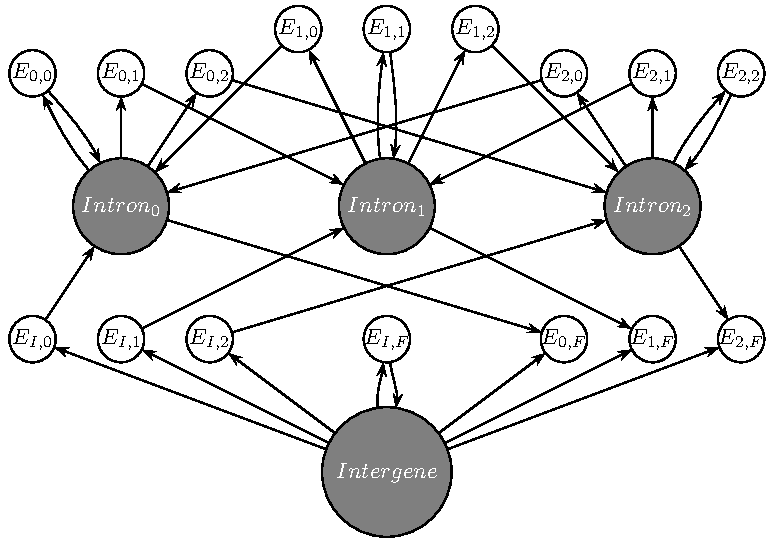
\includegraphics{../figures/slam.pdf}
\end{center}
\caption[HMM topology of SLAM's GpHMM]{
Topology of GpHMM used by SLAM (states for genes on reverse strand are omitted).
Gray states has self-loops, which are omitted from the Figure.
Emissions of shaded states are modeled by the basic
three state pHMM. White states represent exons. Each has associated a duration
distribution and emissions are  modeled by three-state pHMM using $5$-th
order states that emit whole codons at once. Since introns can be inside a
codon, the model contains an exon state for every possible interruption:
$E_{i,j},0\leq i,j<3$ is an exon that begins with end of the interrupted codon of
length $((3-i)\mod 3)$ and ends with the start of a codon of length $j$. $I$
stands for start codon and $F$ stand for stop codon.  $Intron_i$ models intron interrupting codon at the
$i$-th position.
}\label{FIGURE:SLAM} \end{figure}

\paragraph{} \firstUseOf{TWAIN} is comparative gene-finder based on GpHMM and
uses intereresting decoding algorithm \cite{Majoros2005}: at first it
independently annotates input sequences using gene-finder TIGRscan
\cite{Majoros2004} finding signals (splice sites, start/stop codons, \dots) and
creating two parse graphs (one for each sequence): signals form vertices
(corresponds to a state of the GpHMM), two signals are connected with an edge
if one can follow other, the probability of an edge is determined by the
probability of the most probable state path between those two states in the
TIGRscan's HMM.

TWAIN then creates graph $G$ by cartesian product of two parse graphs, omitting
the vertices corresponding to pairs of different signals. Each node in the
graph corresponds to a state of the GpHMM and a cell in the dynamic programming
matrix of the Viterbi algorithm.  Edges between cells correspond to an
alignment generated by a single state from GpHMM.  The Viterbi algorithm is
computed only on cells corresponding to graph $G$ which significantly reduces
running time \cite{Majoros2005}.

\paragraph{}
\firstUseOf{GeneWise} predict genes by aligning a protein  to similar gene
structures in DNA \cite{GeneWise2004}. It uses probabilistic transducers
instead of pHMM.  Both transducers and pHMM are probabilistic finite state
machines, but probabilistic transducers transform one sequence into the other
sequence.  It is easy to compose transducers, while maintaining probabilistic
interpretation of the resulting model. Composition of two transducers $A$ and
$B$ is transducer $C$ that that on the input sequence applies transducer $A$
and then transducer $B$.

GeneWise model was created by composition of a gene prediction model $S$ which
translates genomic sequence to protein sequence and a protein homology model $T$
which maps protein sequence to a homologous protein sequence.

Gene prediction model $S$ consists of a single exon state which translates
series of codons into amino-acids, and three submodels for modeling introns.
Protein homology model $T$ is a simple pHMM from figure \ref{FIGURE:SIMPLEPHMM}
defined over protein alphabet \cite{GeneWise2004}.

\paragraph{}

\begin{figure}
\begin{center}
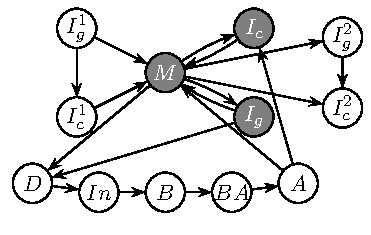
\includegraphics{../figures/pairagon.pdf}
\end{center}
\caption[Topology of Pairagon generalized pair hidden Markov model.]{
Topology of Pairagon GpHMM. All states except states
$D,B$ and $A$ have a self-transition.
Shaded states corresponds to exons: $M$ emits
aligned pairs of symbols, $I_c$ is insertion in the cDNA and $I_g$ is
insertion in the genome. States $I^1_c,I^1_g,I^2_c$ and $I^2_g$ corresponds to
unaligned parts of the DNA and cDNA in the beginning and the end of the
sequences. States $D, In, B, BA, A$ correspond to intron structure:
Donor, Intron, Branch, Branch Acceptor, and Acceptor.
}\label{FIGURE:PAIRAGON}
\end{figure}


The aim of \firstUseOf{Pairagon} is to find local alignments of \abbreviation{complementary
DNA}{cDNA} and genome \cite{Pairagon2009}, By aligning experimentally obtained
cDNA sequences to the genome we are able to confirm intron and exon structures
of genes.  Pairagon's HMM model consists of a simple pair HMM submodel, which
aligns cDNA to DNA and a $5$-state submodel for intron structures. The whole
topology is in figure \ref{FIGURE:PAIRAGON}. 

\begin{comment}
Model was trained using iterative maximum likelihood approach.  Initial
parameters were trained on the alignments from the \abbreviation{Mammalian Gene
Collection}{MGC}. In this phase, the parameters for intron submodel were set by
hand. The model was then used to align more MGC sequences. Final parameters were
estimated from the new alignments.
\end{comment}

Decoding was done by the Viterbi algorithm. Runtime of the algorithm was
improved by the stepping-stone algorithm described in Section \ref{SECTION:SSA}
and memory requirements were improved using the Treeterbi algorithm
\cite{Keibler2007}, which is similar to the On-line Viterbi algorithm \cite{Sramek2007}.

\subsection{Non-Geometric Indel Models}
In the simple pHMM described in figure \ref{FIGURE:SIMPLEPHMM}, gap length has
geometric distribution: the probability that a gap has length $n$ is
$e_{M,I}e_{I,I}^{n-1}(1-e_{I,I})$ (note that the probability that at particular
position will be gap with length zero is $1-e_{M,I}$). The Viterbi
algorithm is usually computed in log-space: instead of computing product of
probabilities of events\footnote{Event is emission or transition.}, we compute
the sum of logarithms of those probabilities, because computation in log-space
is numerically more stable. The Viterbi algorithm for the simple HMM
will become the same as the Needleman-Wunsch algorithm.  Gap penalty will be
$\log(e_{M,I})+\log(1-e_{I,I})+(n-1)\log(e_{I,I})$. By setting $d=\log(e_{I,I})$
and $g=\log(e_{M,I})+\log(1-e_{I,I})-d$ we see that this is exactly affine gap
penalty. Therefore we can say that affine gap penalties correspond to geometric
distribution of indel lengths.

Using non-affine gap model can improve alignment quality.  Problem with
geometric distribution (or affine gap penalties) it that they are not realistic
\cite{Cartwright2009,Lunter2008}.  Therefore some other distribution might be
more appropriate, for example zeta distribution \cite{Cartwright2009}, or
combination of several geometric distributions to approximate the distribution
of gap length \cite{Gill2004,Gill2006}.

GpHMM allow us to use arbitrary duration distributions.  On the other hand,
GpHMM are much slower to decode.  One way of incorporating a different gap
distribution into pair hidden Markov models without using their generalized
version is to use several (for example two) indel states for every sequence. For
example Lunter {\it et al. (2008)} used two component mixture models: instead of
one indel state for every sequence they use two. They report that this improved
quality of alignments. Similar approach is used in the multiple sequence aligner
FASTA \cite{Bradley2009}. \nocite{Lunter2008}

Modeling non-geometric distributions with several states can be problematic when
used with the Viterbi decoding \cite{Vinar2005}. Set of states with the same
emission distribution used for modeling non-geometric distribution is called
gadget. We discuss an example of such a problem for the two component mixture
model.

\begin{figure}
\begin{center}
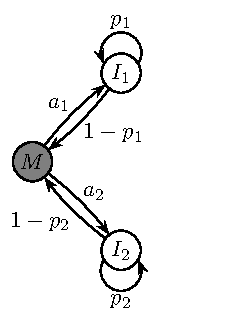
\includegraphics{../figures/twoComponentMixtureModel.pdf}
\end{center}
\caption[The example of an HMM modeling two component geometric distribution]{
Shaded state $M$ represents the match state and states $I_1$ and $I_2$
represents indel states in the same sequence. Indel states for the other
sequence are omitted.
}\label{FIGURE:TWOCOMPONENT}
\end{figure}

Let $H$ be a simple pair hidden Markov model with two pairs of indel states.
Let $I_1$ and $I_2$ be indel states that generate gaps in the first sequence
connected with match state $M$ as in the figure \ref{FIGURE:TWOCOMPONENT}.  Gaps
in alignments (in the first sequence) that are generated by such a model have
length distribution $d(n)=(a_1p_1^{n-1}(1-p_1)+a_2p_2^{n-1}(1-p_2)), n>0$ and
$d(0) = 1-a_1 - a_2$ where $n$ is the length of the gap ($n=0$ means that there
is no gap), $a_1$ and $a_2$ are probabilities of entering state $I_1$ and $I_2$
respectively and $p_1$ and $p_2$ are probabilities of remaining in state $I_1$
and $I_2$ respectively.  This is equivalent to the generalized pair hidden
Markov model $H'$ with one indel state for every sequence which has
$d'(n)=d(n)/(1-d(0))$ as its duration distribution (in generalized states we
want to generate at least one gap. The $d(0)$ should by modeled by the
probabilities of incoming and outgoing transitions to the generalized state). Both models define the same
distribution of alignments  and running the Forward-Backward algorithm or the
Forward algorithm will give the same results. However, alignments constructed by
the Viterbi algorithm can be different for $H$ and $H'$.

Problem is that in the generalized model the Viterbi algorithm gaps of length
$n$ have ``score'' $d(n)$ but in the non-generalized pair hidden Markov model it
will be $m(n)=\max\{a_1p_1^{n-1}(1-p_1),a_2p_2^{n-1}(1-p_2)\}, n>0$ and
$m(0)=1-a_1-a_2$.  These two scores are different ($d(n)$ is always higher) and
therefore it is possible that the Viterbi algorithm reconstruct different
alignments. Therefore if we are using the Viterbi algorithm, we should either
construct a gadget so that $m'(n)$ will be a better approximation of $d(n)$
($d(n)$ is the distribution for the original model) or use a generalized pair
hidden Markov model for the Viterbi algorithm.

%co chcem povedat: niekedy je lepsie pouzit iny gapmodel -- jeden pre kratke
%gapy, jeden pre slhe gapy. Preto sa niekedy 

\subsection{Aligning Sequences with Variable Rate of Evolution}
\label{SECTION:FEAST} 
%\subsection{FEAST} 

The rate of evolution (the expected number of substitution per position in
sequence over some period of time) is not constant for the whole genome. It does
not have to be constant even within one gene. FEAST is pairwise local alignment
tool \cite{FEAST2011} that takes into account the variable evolution rate. The
simple pHMM from figure \ref{FIGURE:SIMPLEPHMM} is optimized for one fixed rate
of evolution.  FEAST contain $k$ such submodels, each trained for a different
rate of evolution.  Submodels are connected with a single silent state.  Since
FEAST is a local alignment tool, it also contains one additional submodel for
generating an unaligned pair of  sequences  at both ends of the sequences.

To construct an alignment (either local or global) FEAST uses the Viterbi
algorithm. Like many local aligners, FEAST uses a seeding heuristics to reduce
computational complexity of finding local alignments.  At first it uses six
different space seeds to get candidate seed and then extends those seeds using
x-drop heuristic \cite{Altschul1997}. The extension is done by an ungapped
version of the Forward algorithm, in contrast with the Viterbi algorithm usually
used for this purpose. 

Estimation of parameters was done by expectation maximization approach (with
Baum-Welsch or Viterbi training). They forced gap parameters to be the same in all
submodels.

Different rates of evolution were also used  in the whole genome aligner GRAPe
\cite{Satija2010}. GRAPe's HMM  consists of two submodels: one with fast
evolution rate and two component geometric mixture model for indels and one with
the lower evolution rate and geometric distribution of indel lengths. GRAPe uses
the Posterior decoding as a decoding method.

\subsection{Biases In Alignments}
\label{SECTION:BIASES}
Lunter {\it et al. (2008)} conducted an extensive survey concerning biases in
alignment. They considered three types of biases associated with gaps. These gap
biases are also discussed in \cite{Durbin1998}. By \firstUseOf{true alignment}
we mean an alignment that corresponds to the actual evolution history.  Since
true alignments are unknown for real data we can simulate evolution on randomly
generated sequences, this obtaining a dataset of ``true'' alignments.

\begin{itemize}[itemsep=-1mm]

\item \firstUseOf{Gap wander} means that a gap is in a different location that in
the true alignment. Is is due to random short similarities around the borders of
gaps that are indistinguishable from true homologies.

\item \firstUseOf{Gap attraction} is occurs when two gaps are near each other.
In such case merging those gaps and introducing a few mismatches might lead to
higher score. 

\item \firstUseOf{Gap anihilation} occurs when there are two gaps of the same
length, one in each both sequence. Since indels are not so common, removing both
gaps while introducing new mismatches might increase the score of an alignment.

\end{itemize}


Biases are ordered by their frequency from the most occurring to the least
occurring \cite{Lunter2008}. Lunter {\it et al.} explore there problems with a
series of simulations.

They measure the alignment quality by \firstUseOf{sensitivity}, which is the
ratio of the correctly predicted alignment columns to all homologous columns in
the true alignment \cite{Lunter2008}. 

\todo{vyhodit cisla?}
In the first experiment, authors use a simple model of evolution obtaining
alignments with the expected sequence identity $0.705$ with geometric gap model.
The sequences were then realigned using the Viterbi algorithm with the same
model as was used for simulation. Sensitivity was lowest for the  columns near
gaps ($56$\%) and the sequence identity for columns near gaps was $85$\% which
does not agree with the expected sequence identity $0.705$\%.  Moving away from
gaps the average sequence identity dropped to  $0.68$\%. The increased sequence
identity near gaps is due to gap wander bias. The gap attraction effect caused
that the number of gaps that are  near each other was lower than the expected
value obtained from the used gap model.

They also run the Viterbi algorithm parametrized by a range of substitution and
indel rates. The highest sensitivity was obtained for the parameters that were
identical to the parameters used for simulation. However, even then the
sensitivity was only $84$\% indicating that even if we have the right evolution
models, some biases in the alignments are inevitable.  

Lunter {\it et al.} also studied the effect of different decoding methods and
different models on the alignment quality. They simulated evolution with
parameters that are close to the parameters of human-mouse evolution. They
simulated for example the large-scale variation of GC content, GC-content
dependent indel and substitution rates and GC-independent local substitution
rate variation \cite{Lunter2008}.  From simulation they obtained $20,000$
homologous sequence pairs with average length of $700$ nucleotides. They add
flanking sequences of length $100$ nucleotides to the generated sequences  to
simulate local alignments.

After simulation they realigned homologous sequences using the Viterbi algorithm
(VA), the Posterior decoding (PD) and the Marginalized posterior decoding (MPD)
with different models: the three state pHMM ($H_S$); $H_S$ with two indel states
for
every sequence  representing the two component geometric mixture gap model ($H_M$) and the
full model with all parameters that were used for simulation ($H_F$).

They also introduce two additional measures of the alignment quality. The
\firstUseOf{false positive fraction (FPF)} is the proportion of the columns that
are ungapped in the true alignment but wrongly aligned by an algorithm
\cite{Lunter2008}. The \firstUseOf{the nonhomologous fraction (NHF)} is the
proportion of columns containing padding sequence among all columns aligned by
an algorithm.


The use of the different models has little impact on the sensitivity of the
constructed alignments. It is interesting that for the Viterbi algorithm the
sensitivity was lower for the full $H_3$ model than for the simple model $H_1$.
This might be explained by the multiple path problem.  With other decoding
algorithms the models $H_2$ and $H_3$ has slightly higher sensitivity then the
$H_1$ model. 

While the use of the ``better'' model does not significantly improve the quality
of alignments, using the Posterior decoding and Marginalized Posterior decoding
improved the sensitivity by approximately $2.5$\% regardless of the model. On
the other hand the FPF and the NHF was increased with use of the PD and MPD. The
sensitivity of the PD and the MPD were similar but the FPF was lower for the MPD
than for PD. 

The main outcome of this experiment is that proper decoding method can improve
the alignment quality while the use of a simpler model doest not significantly
reduce the alignment quality. However, Lunter {\it et al.} use in their
simulations models only relatively simple models of the evolution. By
incorporating information about gene stricture into alignment models combined
with the use of the right decoding algorithm we can improve alignments further.
This will be discussed in the next chapter. 



\section{Algorithmic improvements}\label{SECTION:ALGORITHMICIMPROVEMENTS}

Needleman-Wunsch algorithm and decoding algorithm for HMMs and pHMMs uses
dynamic programming. In this section we review several algorithmic improvements
to these algorithms. Some of the techniques will not be universally applicable.
With these techniques, alignment algorithms could be used with sequences much
longer than several thousand bases.

\subsection{Restricting Search Space}

One commonly used technique for speedup (and decreasing memory requirements) of
sequence alignment is to restrict the search space of dynamic programming. We
compute alignment only in some parts of matrix $M$ and we assume that omitted
parts of matrix correspond to alignments with low score. These techniques are also 
applicable for pHMMs.

If the two sequences are quite similar, the optimal global alignment will not
be too far from the main diagonal of matrix $M$. Therefore it is not necessary
to compute parts of matrix $M$ that are too far from the main diagonal
\cite{Chao1992} (distance from diagonal a is user-defined value or can be
computed during alignment \cite{GusfieldBook}).  However, this method is not
useful for local alignment or global alignment of distant sequences. Now we
will discuss some more advanced techniques to restricting search space of
dynamic programming.

\subsubsection{Seeds}

Seeds are a technique frequently  used to reduce time complexity of local
alignment.  They were popularized by BLAST algorithm \cite{Altschul1990}.  A
\firstUseOf{seed} is a short alignment which is likely to be a part of an
alignment with high score. After a seed is found, it is extended with an
extension algorithm to a local alignment.

Seeds that cannot be extended to high-scoring alignments are discarded. Such
candidate seeds are called false positives.  Alignments that were not found by
our heuristics are called false negatives.  It is important that heuristics
used to find seeds has a small number of false negatives and a large number of
true positives, otherwise many true high-scoring local alignments will not be
found. On the other hand, high number of false positives implies longer running
time. 


The most traditional approach is to take as seeds all pairs of positions $i$
and $j$, such that $X[i:i+\tau]=Y[j:j+\tau]$ for some
constant $\tau$. This approach is used in BLAST \cite{Altschul1990}.  Various
generalization were developed to improve trade off between
speed and accuracy, such as seeds with mismatches \cite{Kent2002}, space seeds
\cite{Ma2002}, vector seeds \cite{Brejova2005vector} or daughter seeds
\cite{Csuros2005}.

Extension of a seed to a full alignment is done in both directions, usually
using equation \ref{ALIGN:ALGO:AFFINE} (equation is altered to reverse
direction). Extension is stopped, when some criterion is reached. For example,
BLAST introduced X-drop heuristics: extension stops if the score of an alignment
is lower than the best score that was seen so far minus some user-defined
constant \cite{Altschul1997}.

\subsubsection{Stepping-Stone Algorithm}
\label{SECTION:SSA}

\abbreviation{Stepping-stone algorithm}{SSA} 
\cite{Meyer2002,Pairagon2009} is suitable for global alignment algorithms. The idea is to
use good local alignments as anchors. An anchor is similar to a seed: it is a
short alignment which we expect to be in the optimal global alignment.
However, local alignment tools give local alignments that do not have to be
consistent with each other. A set of local alignments is consistent if all
local alignments can be together in one global alignment.

SSA chooses a consistent set of local alignments  by a simple greedy method,
always adding highest-scoring alignment consistent with those selected so far.
Selected anchors will be extended to a global alignment. However, since local
alignments may contain errors, SSA will relax them. If $X_i$ and $Y_j$ were
aligned in some anchor, then $X_i$ can be aligned to positions from $j-\tau$ to
$j+\tau$ in the global alignment\footnote{Or aligned to a gap in that region.}
for some user defined constant $\tau$. Similarly, $Y_j$ can be aligned to
positions from $i-\tau$ to $i+\tau$. This technique is also called \firstUseOf{banding},
and it is often used. We used this technique in chapter \ref{CHAPTER:REP}.

\subsection{Reducing memory complexity}
One general technique to reduce the memory requirements of dynamic programing
is \firstUseOf{checkpointing} \cite{Grice1997}.

In order to compute the $i$-th row of matrix $M$, we need only row $i-1$. As
mentioned in section \ref{SECTION:NEEDLE}, to compute the score of the best
alignment we need to store only
two consecutive rows.  However, if we want to
recover the optimal alignment, after we have computed its score, we need all
rows of matrix $M$ again, in decreasing order.

Checkpointing solves this problem by storing every $k$-th row of matrix $M$,
$\lceil n/k\rceil$ rows in total.  While back-tracing, we will remember an
additional block $B$ of consecutive $k$ rows in interval $[ik,(i+1)k)$. We can
compute such a block in $O(kn)$ time using the basic dynamic programming,
starting from row number $ik$ which is stored in memory.  Overall, we recompute
every block at most once, and therefore the time complexity will be $O(mn)$.
If we set $k=\sqrt n$ then the memory complexity will be $O(m\sqrt n)$. By
using $l$ recursive applications of this technique we can obtain algorithm with
memory complexity $O(m\sqrt[l]{ n})$.

Even more space reduction can be obtained using the Hirschberg algorithm \cite{Hirschberg1975}. The idea is
the following: if we want an alignment of sequences $X$ and $Y$ that has bases $X_i$
and $Y_j$ aligned, we have to  do dynamic programming only in submatrices
$M_1=M[0:i,0:j]$ and $M_2=M[i:n-1,j:m-1]$. If $i=\lceil n/2\rceil$ then
the total number of cells in those matrices is roughly half of the number of
cells in $M$. The Hirschberg algorithm incorporates a procedure to compute 
$j$ such that $X_i, i=\lceil n/2\rceil$ is aligned to $Y_j$ in optimal alignment of both sequences in $O(nm)$
time and $O(n+m)$ memory. If $X_i$ is aligned to a gap, it finds $j$ such
that $X_i$ is aligned to gap that comes right after $X_j$.
The algorithm then uses such $j$ to determine submatrices $M_1,M_2$ and finds alignments in them recursively.
The optimal alignment is a concatenation of optimal alignments in matrices $M_1$ and
$M_2$.

Since total size of the two subproblems is always at most half of the size of
the original problem, the running time of the algorithm will be roughly double
of the standard dynamic programming.  The Hirschberg algorithm keeps in memory
only a constant number of rows of $M$,  and therefore the memory requirements
are $O(n+m)$. The Hirschberg algorithm reduces memory more than checkpointing,
but checkpointing can be applied to a wider class of algorithms. 
Checkpointing can be used to decrease the memory complexity of the Viterbi
algorithm with back-tracing procedure and the Posterior decoding to $O(\sqrt n
m)$.  Similarly, this technique can be used to reduce memory complexity of the
algorithms for pHMMs to $O(nm\sqrt n )$ where $n$ is the length of the longer
sequences and $m$ is the number of states of HMM.

\subsubsection{The Viterbi Algorithm}
As we described in section \ref{SECTION:VITERBI}, in the Viterbi algorithm we compute values
$V[i, v]$ (the probability of the most probable state path ending in state $v$
and generating the prefix of the input sequence of length $i$) and $B[i, v]$
containing the previous state in the most probable state path, which is used in
back-tracing.

While back-tracing, we need access to values of matrix $B$ in decreasing order.
We need only matrix $B$ and last row of $F$. From $i$-th row of $F$ we can
recompute $i+1$-th row of $B$. Therefore we will remember every $k$-th row of
$V$ from which we will recompute blocks of matrix $B$. $B$ will be split into
blocks $B_0=B[1:k+1,:],B_1=[k+1:2k+2,:],\dots,B_i=B[ik+1:{i+1}k+1,:],\dots$ We
will keep in the memory exactly one block of $B$. If we need row that is in
block $B_i$ but $B_i$ is not in memory, we discard current block and compute
block $B_i$ from $V[ik,\cdot]$. Since we need rows of $B$ in decreasing order,
we recompute every block exactly once. If $k=\theta(\sqrt n)$ then the memory
complexity is  $O(n+m\sqrt n)$.

For two dimensional version we keep every $k$-th matrix $V[ik,\cdot,\cdot]$.
Algorithm is analogous to one-dimensional version or to the checkpointing
technique for the Needleman-Wunsch algorithm


\subsubsection{The Posterior Decoding}

In the Posterior decoding need to interlace computations of $F[i,v]$ and
$B[i,v]$ to compute $F[i,v]\cdot B[i,v]$ for all $0\leq i<n,v\in V$. We will
compute $F$ using the checkpointing technique (we compute every $k$-th row of
$F$ and keep in memory only one block).  $B[i,v]$ will be computed row by row
with the version of the  Backward algorithm that need only $O(m)$ memory. When
we compute $B[i,v]$, we also compute $F[i,v]$ by checkpointing technique (if $i$ is in
current block then return $F[i,v]$ from current block. Otherwise discard current
block and recompute the block for row $i$). With this approach we can
compute the posterior values with the $O(m\sqrt n)$ memory. We recompute every row at most
once and therefore the time complexity is $O(n(m+t))$.

\subsection{Exploiting Sequence Repetition}

There are two similar techniques to accelerate sequence alignment. Both divides
the dynamic programming matrix into blocks (square of rectangle submatrices).
Each block has input and output cells. Input cells are in the left and bottom
border of the submatrix and output cells are in the top and right border of the
submatrix (if the computation is performed in top-right order). Each submatrix
transforms the input cells into output cells (the computation of dynamic
programming). It is possible to use either compression or pre-computation to
compute alignment in time proportional to the total length of the borders of
the blocks instead of the total size of the block (block of size $t\times u$
has border length $O(t+u)$ and size $O(tu)$).

The first such technique is called Four-Russian technique \cite{Arlazaroff1970,
GusfieldBook} and can be used for computing edit distance or sequence alignment
with some restriction of the scoring matrix. It divides the dynamic programming
matrix into equally sized blocks and pre-computes the output cells for all
possible input cells and all possible blocks (the differences between values of
the input cells are small, so all possible inputs can be enumerated). By
setting the block size to the $O(\log(n))$, the total running time of the
algorithm is $O(n^2/log(n)^2)$ in the unit-cost model \cite{GusfieldBook}.

Instead of dividing matrix into equally sized submatrices, we can run LZ78
factorization \cite{Lempel1976} on both sequences.  LZ78 factorization is
compression technique which divide sequence into sequence of $O(n/log(n))$
segments, where each segment $s$ has predecessor segment $s_p$, where $s=s_pc$,
$c$ is a single character. We can use these segments to construct blocks. Each
of such blocks has three predecessors blocks that are obtained by using
predecessor segments \cite{Crochemore2002}. Crochemore {\it et al.} developed
technique to compute the values of the output cells from the predecessor blocks
and input cells in $O(b)$ time where $b$ is the total border length of the
block. It utilizes the $O(A+B)$ algorithm for computing row minima/maxima in
totally a monotone matrix of size $A\times B$ \cite{Aggarwal1987}.  The total
time complexity of this algorithm is $O(n^2/\log n)$ time
\cite{Crochemore2002}.

Similar idea was also used for accelerating dynamic programming for decoding
and training of HMMs \cite{Weimann2009}. The computation of the Forward
algorithm can be decomposed as an series of matrix multiplication. Using LZ78
factorization, we can divide this into multiplication of $n/\log(n)$, where
multiplication of matrices in each block is done in $O(m^3)$ where $m$ is the
number of states of HMM. Using this, we can compute the Forward algorithm in
$O(nm^3/log(n))$ time which lead to $O(\log(n)/m)$ speed-up \cite{Weimann2009}.
Similarly, it is possible to use this technique to the Viterbi algorithm. In
this case we replace summation with maximum in the matrix multiplication
operation \cite{Weimann2009}.
